
\section{Issues and motivations}

Causal broadcast is a communication primitive that allows a process to send
messages to all processes of its distributed system (\REF). Message deliveries
follow the happen before relationship (\REF). If the sending of a message $m$
precedes the sending of a message $m'$ then all processes that deliver these two
messages need to deliver $m$ before $m'$. Otherwise they deliver them in any
order. Each process may receive a message multiple times but it delivers it
exactly once.

\PCBROADCAST (\REF) is a causal broadcast where broadcast messages piggyback
constant size control information. The overhead brought by causal order in terms
of generated traffic is negligible.  \PCBROADCAST uses FIFO communications links
and forwarding for causal broadcast (\REF); while sending few control messages
to handle dynamicity (see Table~\ref{table:complexity}).

\begin{figure*}
  \begin{center}
    \subfloat[Part A][\label{fig:spaceproblemA}Process~B broadcasts $b$ along
    with control information $\langle B,\,1 \rangle$.]
    {\input{input/figspaceproblemA.tex}}
    \hspace{10pt}
    \subfloat[Part B][\label{fig:spaceproblemB}Process~A receives, saves in its
    local vector, delivers and forwards
    $b$. Process~B wants to add Process~C in its direct neighbors for
    causal broadcast. It sends a control message $\pi$ to Process~C using 
    Process~A as mediator.]
    {\input{input/figspaceproblemB.tex}}    
    \hspace{10pt}
    \subfloat[Part C][\label{fig:spaceproblemC}Process~A broadcasts $a$ along with
    control information $\langle A,\, 1 \rangle$. Then, it routes $\pi$ towards
    Process~C. Process~B receives $b$ but discards it, for it is already
    registered in Process~B's local vector.]
    {\input{input/figspaceproblemC.tex}}
    \hspace{10pt}
    \subfloat[Part D][\label{fig:spaceproblemD}Process~B and Process~C receive,
    save in their local vector, deliver and forward $a$. In addition, Process~B
    buffers $a$ to send it later to Process~C.]
    {\input{input/figspaceproblemD.tex}}
    \hspace{10pt}
    \subfloat[Part E][\label{fig:spaceproblemE}Process~C receives $\pi$ and 
    replies $\rho$ to Process~B.]
    {
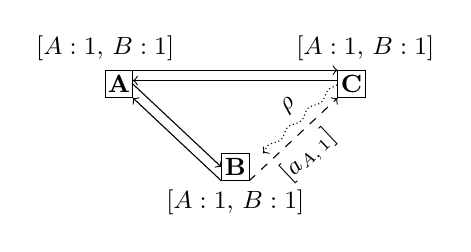
\begin{tikzpicture}[scale=1]
  
  \small
  
  \newcommand\X{210/5pt};
  \newcommand\Y{30pt};

  
  \draw[fill=white] (0*\X, 0*\Y) node{\textbf{A}} +(-5pt, -5pt) rectangle +(5pt, 5pt);
  \draw (-5+0*\X, 5+0*\Y) node[above]{$[A:1,\,B:1]$};
  \draw[fill=white] (1*\X, -1*\Y) node{\textbf{B}} +(-5pt, -5pt) rectangle +(5pt, 5pt);
  \draw (1*\X, -5-1*\Y) node[below]{$[A:1,\,B:1]$};
  \draw[fill=white] (2*\X,  0*\Y) node{\textbf{C}} +(-5pt, -5pt) rectangle +(5pt, 5pt);
  \draw (5+2*\X, 5+0*\Y) node[above]{$[A:1,\,B:1]$};
  
  \draw[->](5+0*\X, 0*\Y) -- 
  (-5+1*\X, -1*\Y); %% A->B

  \draw[<-](5+0*\X, -5+0*\Y) --
  (-5+1*\X, -5-1*\Y); %% A<-B
  
  \draw[->](5+0*\X, 5+0*\Y) --
  (-5+2*\X, 5+0*\Y); % A->C
  
  \draw[<-](5+0*\X,  1.25+ 0*\Y) --
  (-5+2*\X,  1.25+ 0*\Y); % A<-C
  
  % \draw[->,dashed](5+1*\X, -1*\Y) -- (-5+2*\X, 0*\Y); %% B<-C
 \draw[<-,densely dotted,decorate, decoration={snake, amplitude=0.3mm}](5+5+1*\X, 5+-1*\Y) -- 
 node[above, sloped]{$\bm{\rho}$}
 (-5+2*\X, 0*\Y);

  \draw[->, dashed](5+1*\X, -5-1*\Y) --
  node[sloped, below]{$[a_{A,\,1}]$} (-5+2*\X, -5+0*\Y); %% B->C



\end{tikzpicture}}
    \hspace{10pt}
    \subfloat[Part F][\label{fig:spaceproblemF}Process~B empties its buffer to
    Process~C. The latter will discard the message $a$, for it is already registered
    in Process~C's local vector]
    {\input{input/figspaceproblemF.tex}}
    \caption{\label{fig:spaceproblem}\PCBROADCAST relies on vectors to deliver
      once and discard multiple receipts. The size of vectors increases linearly
      with the number of processes that ever broadcast a message.}
  \end{center}
\end{figure*}

Figure~\ref{fig:spaceproblem} depicts its functioning while highlighting the
problem. In this scenario, the system comprises 3 processes. At first, Process~B
cannot communicate directly with Process~C. In Figure~\ref{fig:spaceproblemA},
Process~B broadcasts $b$. It assigns it a unique identifier
$\langle B,\, 1 \rangle$ and saves this element in a local vector. In
Figure~\ref{fig:spaceproblemB}, Process~A receives $b$. Its vector does not
contain this element. Hence, Process~A saves $\langle B,\,1\rangle$ in its
vector, delivers and forwards $b$. In the meantime, Process~B wants to add a
direct communication link to Process~C for causal broadcast. For the sake of
safety, i.e., sending messages using this new link cannot violate causal order,
Process~B must send a control message $\pi$ to Process~C using already
established link. It uses Process~A as mediator and buffers its delivered
messages while awaiting for Process~C's reply. In
Figure~\ref{fig:spaceproblemC}, Process~A broadcasts $a$ along with its assigned
unique identifier $\langle A,\, 1 \rangle$. Process~A updates its local vector
accordingly. Then, Process~A routes $\pi$ to Process~C. Process~B receives $b$
but discards it, for its local vector already contains this message.  Process~C
receives, saves, delivers, and forwards $b$. In Figure~\ref{fig:spaceproblemD},
Process~A receives and discards $b$. Process~B receives, saves, delivers,
buffers, and forwards $a$. Process~C receives, saves, delivers, and forwards
$a$. In Figure~\ref{fig:spaceproblemE}, Process~A receives two copies of an
already delivered message $a$, hence discards them both. Process~C receives
$\pi$ and sends its reply $\rho$ to Process~B. Such reply can travel using any
communication mean. In Figure~\ref{fig:spaceproblemF}, Process~B receives
$\rho$. Process~B empties its buffer comprising $a$ to Process~C. This procedure
ensures that the delivery of $b$ happens before the delivery of $a$ at
Process~C. Afterwards, Process~B uses this link normally for causal broadcast.

This scenario highlights the issue about memory consumption: the local structure
to discards multiple receipts increases linearly with the number of processes
that ever broadcast a message.

\begin{figure*}
  \begin{center}
    \subfloat[Part A][\label{fig:counterproblemA}Process~B broadcasts the 
    message $b$ and expects to receive 1 copy of $b$.]
    {\input{input/figcounterproblemA.tex}}
    \hspace{10pt}
    \subfloat[Part B][\label{fig:counterproblemB}Process~A receives, delivers
    and forwards $b$. It expects 1 additional copy of $b$. Process~B wants to 
    add Process~C in its direct neighbors for causal broadcast. It sends a 
    control message $\pi$ to Process~C using Process~A as mediator.]
    {\input{input/figcounterproblemB.tex}}
    \hspace{10pt}
    \subfloat[Part C][\label{fig:counterproblemC}Process~A broadcasts $a$. It 
    expects 2 copies. Process~B receives $b$ again, it does not expect any other 
    copy. Hence, it purges its local structure from $b$. Process~C receives, 
    delivers and forwards $b$. It does not expect additional copies.]
    {\input{input/figcounterproblemC.tex}}
    \hspace{10pt}
    \subfloat[Part D][\label{fig:counterproblemD}Process~A receives, discards,
    and purges $b$. Process~B and Process~C receive, deliver, and forward $a$ but
    do not expect any additional copy. Process~B buffers $a$ to ensure the safety 
    of the new link.]
    {\input{input/figcounterproblemD.tex}}
    \hspace{10pt}
    \subfloat[Part E][\label{fig:counterproblemE}Process~A receives and discards 
    two copies of $a$. It purges its local structure of $a$. Process~C receives
    $\pi$ and replies $\rho$ to Process~B.]
    {\input{input/figcounterproblemE.tex}}
    \hspace{10pt}
    \subfloat[Part F][\label{fig:counterproblemF}Process~B empties its buffer
    to Process~C. Not only Process~C mistakes $a$ for a new message and delivers it 
    again, but it has cascading effects due to the forwarding.]
    {\input{input/figcounterproblemF.tex}}
    \caption{\label{fig:counterproblem}Using counters to discard multiple receipts
      is more efficient in terms of memory usage but fails in dynamic systems.}
  \end{center}
\end{figure*}

However, we observe that information about messages becomes obsolete over
receipts. For instance, all copies of the message $b$ disappear of the system in
Figure~\ref{fig:spaceproblemD}. With such knowledge, processes could remove this
message from their local structure safely. 

Figure~\ref{fig:counterproblem} depicts the same scenario where we replace the
linearly increasing local structure by a set of messages purged over
receipts. Assuming that each process delivers and forwards each message exactly
once, processes expect to receive one copy of each broadcast message per link
pointing to them. For instance, in Figure~\ref{fig:counterproblemA}, Process~B
expects to receive one copy of $b$, for only Process~A has Process~B as
neighbor; in Figure~\ref{fig:counterproblemC}, Process~A expects two copies of
$a$, for both Process~B and Process~C have Process~A as neighbor. Received
messages that are not in the local structure are new and must be
delivered. Receives messages that are in the local structure must be ignored and
the counter of expected copies decremented. When this counter reaches 0, the
process assumes that it will not receive this message again, hence it purges its
local structure from this message. For instance, in
Figure~\ref{fig:counterproblemC}, Process~B removes the element $b$, for it
received the awaited copy; in Figure~\ref{fig:counterproblemE}, Process~A
removes the element $a$, for it received both awaited copies.  Unfortunately, in
Figure~\ref{fig:counterproblemF}, the number of expected messages becomes
inconsistent due to dynamicity. Process~B empties its buffer of messages
containing $a$, for the sake of causal order. When Process~C receives $a$, it
mistakes this message for a new message. Not only Process~C delivers $a$ a
second time, but it forwards it to its neighbors leading to a cascading effect
of multiple deliveries.

%Process~C was unable to distinguish messages it would receive from Process~B
%(i.e., $a$) from messages it would never receive from Process~B (i.e., $b$).

Even if counters are insufficient to discard multiple receipts in dynamic
systems, this hints that broadcast can guarantee reliability locally without
maintaining costly data structures summarizing the global state of the system,
e.g., using vector clocks.


% To solve this issue, state-of-the-art protocols maintain a local vector the size
% of which increases linearly with the number of processes that ever broadcast a
% message. They eventually become overcostly in dynamic settings.


In this paper, we exploit and extend \PCBROADCAST to provide a causal broadcast
middleware that is lightweight in terms of local memory consumption, and message
overhead. Table~\ref{table:complexity} shows the complexity of the proposed
approach. It keeps constant message overhead and constant delivery execution
time while removing the linear dependency $N$ from the local space
complexity. Its overhead in terms of number of control messages is twice that of
\PCBROADCAST.
%% It maintains a local structure that grows and shrinks over time when
%% processes can join, leave, or self-reconfigure their neighborhood over time.
%% \TODO{maybe more details.}
The next section describes the proposed protocol.


%%% Local Variables:
%%% mode: latex
%%% TeX-master: "../paper"
%%% End:
